\chapter{Enrichment of SAC proteins at kinetochores strengthens the SAC signaling}
\label{chpt:3}

The model which we proposed in \myref{ProzoneEffectModel} relies on certain basic assumptions. First, the competition among a large but physiologically relevant number of phosphorylated MELT motifs for the limited pool of SAC proteins can effectively diminish freely diffusive SAC proteins in the cytosol. Second, the co-localization of multiple SAC proteins on the same \protein{Knl1} scaffold cooperatively boosts the SAC signaling activity. Our follow-up studies described in this chapter aimed to prove these assumptions in a kinetochore-based setting.

This chapter is tailored from two of my first-author manuscripts (submitted to a peer-reviewed scientific journal or under review) with the inclusion of unpublished supplementary data (\myref{HybridGenotypingdsDNA,5RACE}). All other figures were reproduced from the two manuscripts and certain statements were adjusted. I was the main contributor of all experiments except those in \myref{SACProteinKinetochoreRecruitment,BUBR1del432-484KTLocalization}, which are credited accordingly in the figure caption.

\section{Using CRISPR-Cas9-mediated genome editing to tag SAC genes with mNeonGreen \Latin{in situ}}

A common practice to study the functions of a protein is to knock down the endogenous protein by RNA interference and then rescue the cells with a mutated or truncated protein ectopically expressed in the cells. This is henceforth referred to as a knockdown-rescue experiment.
%Transient transfection may offer poor consistency in the expression level across different cells or throughout a long time course.
This strategy may cause undesirable over-expression of SAC proteins, which affects the progression of mitosis \cite{Bub1Overexpression-AuroraBHyperactivation} (see also \myref{per_se}), depletes the cytosolic pool of the corresponding binding partner and impairs the SAC signaling activity \cite{Bub3Competition, FissionYeastSACRobustness, ATMPhosphorylatesMad1S214, MAD1Overexpression_Ryan2012}, or even induces cell death (our unpublished imaging data of HeLa-A12 cells).
% 20160614_pPS28_Bub1_BubR1_Cdc20 (IncuCyte data) or my BubR1-rescue time-lapse experiments on the left scope

Therefore, we utilized CRISPR-Cas9-mediated genome editing to tag SAC genes \Latin{in situ} \cite{HDRTiming}, which may better protect any endogenous transcriptional and translational regulations by preserving the introns or the 5'/3'-untranslated regions (UTRs; see \myref{5RACE}). This chapter focuses on three proteins from different layers of the SAC recruitment cascade: \protein{Bub1}, \protein{BubR1}, and \protein{Mad1}. We fused mNeonGreen to the N-terminus (upstream of the first exon) of \gene{BubR1} and \gene{Bub1} as well as the C-terminus (downstream of the last exon and before the stop codon) of \gene{Mad1} to enabled live-cell fluorescence imaging. We chose to tag \gene{Mad1} at its C-terminus based on a previous report that large N-terminal tags may disrupt the localization of \protein{Mad1} to the corona \cite{CoronaActivatesSAC}. mNeonGreen is separated from the tagged protein by a short flexible linker (see \myref{CRISPRMethods}) so that the binding dynamics, functions, and turnover of the protein may be minimally affected. mNeonGreen has fast maturation kinetics (shorter than \SI{10}{min} at \SI{37}{\celsius} \cite{mNG}) compared to the turnover rates of \protein{BubR1} and \protein{Bub1} in nocodazole-arrested mitotic cells \cite{BubR1MitosisTurnover, Bub1MitosisTurnover}. These CRISPR-Cas9-edited cell lines can also serve as a reference for the endogenous expression of these SAC proteins for knockdown-rescue experiments (\myref{NewBUBR1Rescue} and the next chapter).

Band intensities from immunoblotting (\myref{WBValidation}) and genotyping PCR (\myref{GenotypingValidation}) suggested that a half of \protein{BubR1} proteins in mitotic mNG-\gene{BubR1} cells and slightly over a half of \protein{Mad1} proteins in mitotic \gene{Mad1}-mNG cells were tagged with mNeonGreen. Our genotyping PCR revealed only one band corresponding to the edited mNG-\gene{Bub1} allele (\myref{GenotypingValidation}). However, immunoblotting using three different antibodies consistently revealed the coexistence of both mNG-tagged and wildtype \protein{Bub1} proteins in mitotic mNG-\gene{Bub1} cells (\myref{siBUB1,simNG-siBUB1}). We suspected that the double-strand break induced by Cas9 may have induced unexpected chromosomal rearrangement at the \gene{Bub1} locus, rendering the ``wildtype'' allele unable to be amplified by the genotyping primers but still able to express the wildtype \protein{Bub1} protein.

To validate this, we conducted 5'-rapid amplification of cDNA ends (RACE) to sequence the 5' region of all \gene{Bub1} mRNAs in the mNG-\gene{Bub1} cells. As a control, We only detected wildtype \gene{Bub1} mRNAs from the parental HeLa-A12 cell line. However, from the mNG-\gene{Bub1} cells, we identified both the mRNA translating into mNG-\protein{Bub1} as well as an mRNA that has an unexpected 5'-UTR (\myref{5RACE}). The open reading frame of this unexpected mRNA still encodes the wild-type \protein{Bub1} protein. The exact configuration of the probable chromosomal rearrangement is unknown because 5'-RACE can only reveal the sequence of the 5'-UTR but not where the genotyping primers are supposed to bind. Nonetheless, this likely explains why the genotyping primers could not amplify the ``wildtype'' allele.

\begin{figure} [b!]
    \centering
    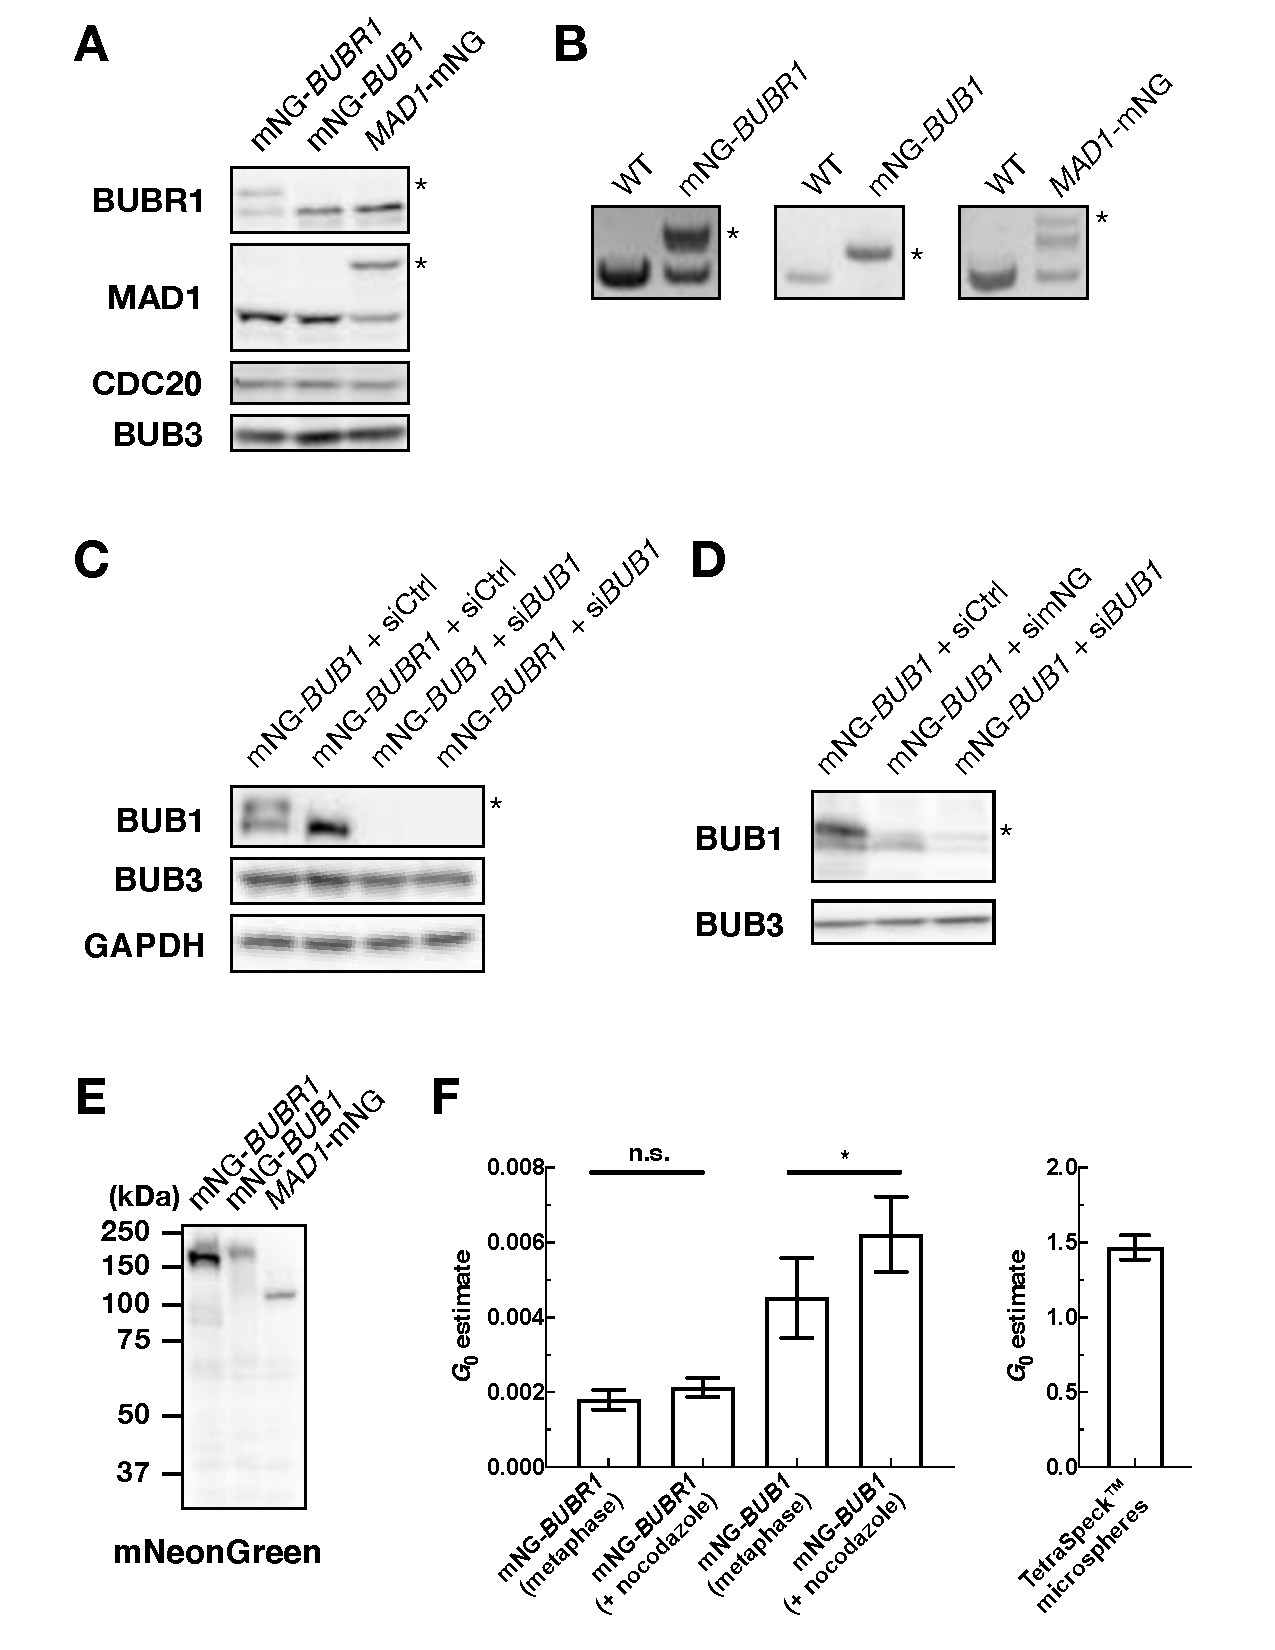
\includegraphics[width=\textwidth]{chapters/figures/CRISPRValidation.pdf}
    \phantomsubfiglabel{WBValidation} % subfigure A
    \phantomsubfiglabel{GenotypingValidation} % subfigure B
    \phantomsubfiglabel{siBUB1} % subfigure C
    \phantomsubfiglabel{simNG-siBUB1} % subfigure D
    \phantomsubfiglabel{anti-mNG} % subfigure E
    \phantomsubfiglabel{FCS} % subfigure F
    \caption{\textbf{Utilizing CRISPR-Cas9-mediated genome editing to fuse mNeonGreen to \gene{BubR1}, \gene{Bub1}, and \gene{Mad1} \Latin{in situ}.}}
    \label{CRISPRValidation}
\end{figure}
\begin{figure} [t!]
    \noindent\justifying \textbf{(Caption of \myref{CRISPRValidation} continued from a previous page)} (A) Immunoblots of mitotic mNG-\gene{BubR1}, mNG-\gene{Bub1}, and \gene{Mad1}-mNG HeLa-A12 cells. Bands marked by asterisks correspond to proteins tagged by mNeonGreen. These blots are representative of three independent experiments. \protein{BubR1} bands were detected by horseradish peroxidase-catalyzed chemiluminescence. \protein{Mad1}, \protein{Cdc20}, and \protein{Bub3} bands were detected by fluorescent dye-conjugated secondary antibodies. \protein{Cdc20} and \protein{Bub3} levels in HeLa-A12 cells were not affected by the \Latin{in situ} tagging of \gene{BubR1}, \gene{Bub1}, or \gene{Mad1}. The weak bands below the strong wildtype bands in the \protein{Mad1} blot likely correspond to the alternatively-spliced \protein{Mad1\textbeta{}} \cite{Mad1beta}. (B) The genotyping (and subsequent sequencing) results verified the expected in-frame fusion of mNeonGreen. Bands marked by asterisks correspond to the mNeonGreen-tagged alleles. The middle bands from mNG-\gene{BubR1} and \gene{Mad1}-mNG cells were hybrid DNAs composed of one strand of the PCR product from the edited allele and one strand of the PCR product from the wildtype allele. These hybrid DNAs were thermodynamically less stable (\myref{HybridGenotypingdsDNA}). Adrienne Fontan also contributed here. (C) Immunoblots using lysates of the mNG-\gene{Bub1} HeLa-A12 cell line and another control genome-edited HeLa-A12 cell line revealed that \protein{Bub1} proteins in the mNG-\gene{Bub1} HeLa-A12 cell line were only partially tagged with mNeonGreen. Cells were treated with thymidine and then nocodazole overnight. The left two lanes were mitotic lysates harvested by mitotic shake-off while the right two lanes were pools of all cells (the fraction of cells in mitosis was significantly lower due to the knock-down of \gene{Bub1}). The immunoblot against \protein{Bub1} here was using a commercial rabbit antibody (see \myref{WBMethods}). (D) Knocking down \gene{Bub1} using a siRNA against mNeonGreen (simNG) or a siRNA against \gene{Bub1} (si\gene{Bub1}) confirmed that the lower band in the immunoblot against \protein{Bub1} is \protein{Bub1} (rather than due to cross-reactivity). The immunoblot against \protein{Bub1} here was using a commercial mouse antibody (see \myref{WBMethods}). We also tested another custom antibody from a previous study \cite{SheepAntiBUB1} and saw similar band patterns, further confirming that the lower band in the immunoblot against \protein{Bub1} corresponded to the wildtype \protein{Bub1}. (E) The majority of mNeonGreen-tagged proteins in mitotic mNG-\gene{BubR1}, mNG-\gene{Bub1}, and \gene{Mad1}-mNG HeLa-A12 cells were full length. The contribution of partial degradation or cleavage products to the fluorescence signal in \myref{FCS} is minor. (F) According to the FCS data, the metaphase concentration of mNG-\protein{BubR1} and mNG-\protein{Bub1} in the corresponding genome-edited HeLa-A12 cell line is $(2.4 \pm 0.4) \times 10^2$ nM and $(1.0 \pm 0.25) \times 10^2$ nM, respectively. Concentration measurements were calibrated by 0.1-\textmu{}m TetraSpeck\texttrademark{} microspheres with a nominal concentration of about \SI{0.30}{nM}. $G_0$, the auto-correlation at the 0-time lag, is inversely proportional to the average number of freely diffusive fluorescent proteins/particles in the excitation volume (see \myref{FCSMethods}). Each error bar represents the mean value $\pm$ the 95\% confidence interval of each group. Results from three independent experiments were compiled.
\end{figure}

\begin{figure}
    \centering
    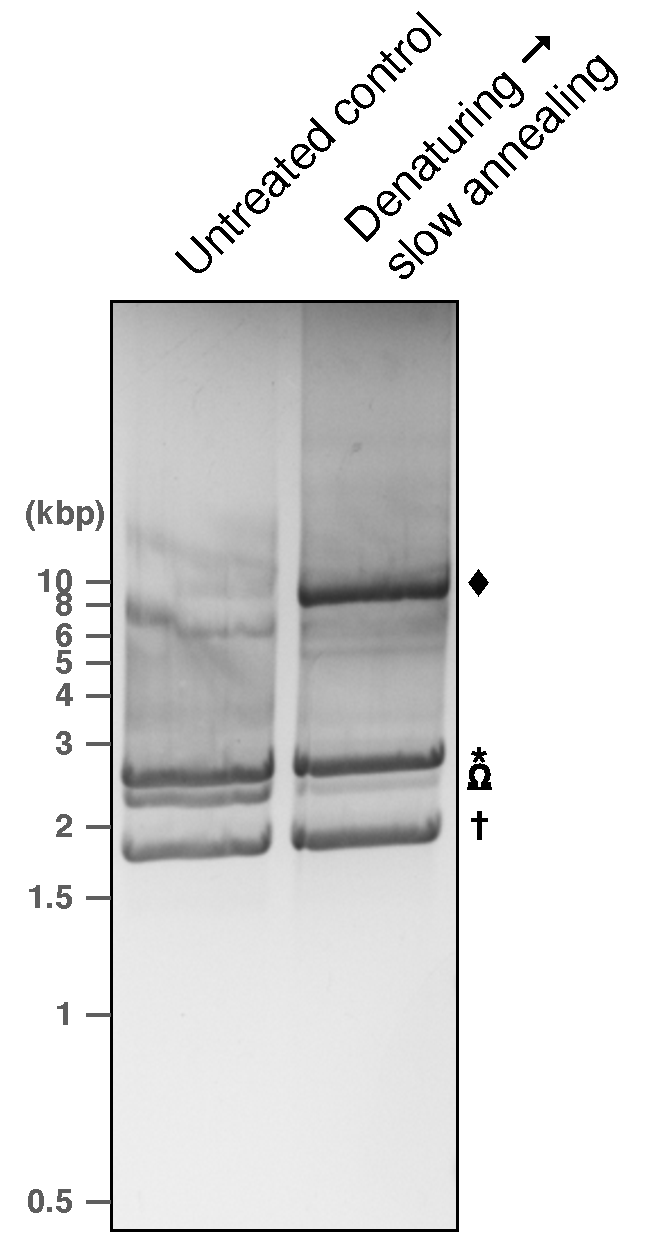
\includegraphics[width=0.3\textwidth]{chapters/figures/HybridGenotypingdsDNA.pdf}
    \caption{\textbf{Genotyping PCR products (using the genome of the heterozygous mNG-\gene{BubR1} HeLa-A12 cell line as the template) feature hybrid double-stranded DNAs that are thermodynamically unfavorable.}}
    \noindent\justifying Genotyping PCR products were purified using the GeneJET PCR Purification Kit (Thermo Fisher Scientific) and then equally split into 2 tubes. One of the tubes (right lane) was then placed in a boiling water bath for \SI{5}{min} and slowly cooled to room temperature, while the other tube (left lane) sit at room temperature. Diamond: likely to be a certain higher-order origami complex. Asterisk: the PCR product of the edited mNG-\gene{BubR1} allele (\SI{2519}{bp}, confirmed by sequencing). Cruciform: the PCR product of the wildtype \gene{BubR1} allele (\SI{1793}{bp}, confirmed by sequencing). \underline{\textOmega{}}: hybrid DNAs made up of one strand from the PCR product of the edited mNG-\gene{BubR1} allele and a complementary strand from the PCR product of the wildtype \gene{BubR1} allele. The identity of this band was also confirmed by sequencing (data not shown). Similar hybrid DNAs likely also existed in the purified \gene{Mad1}-mNG genotyping PCR products \myref{GenotypingValidation}.
    \label{HybridGenotypingdsDNA}
\end{figure}

\begin{figure} [b!]
    \centering
    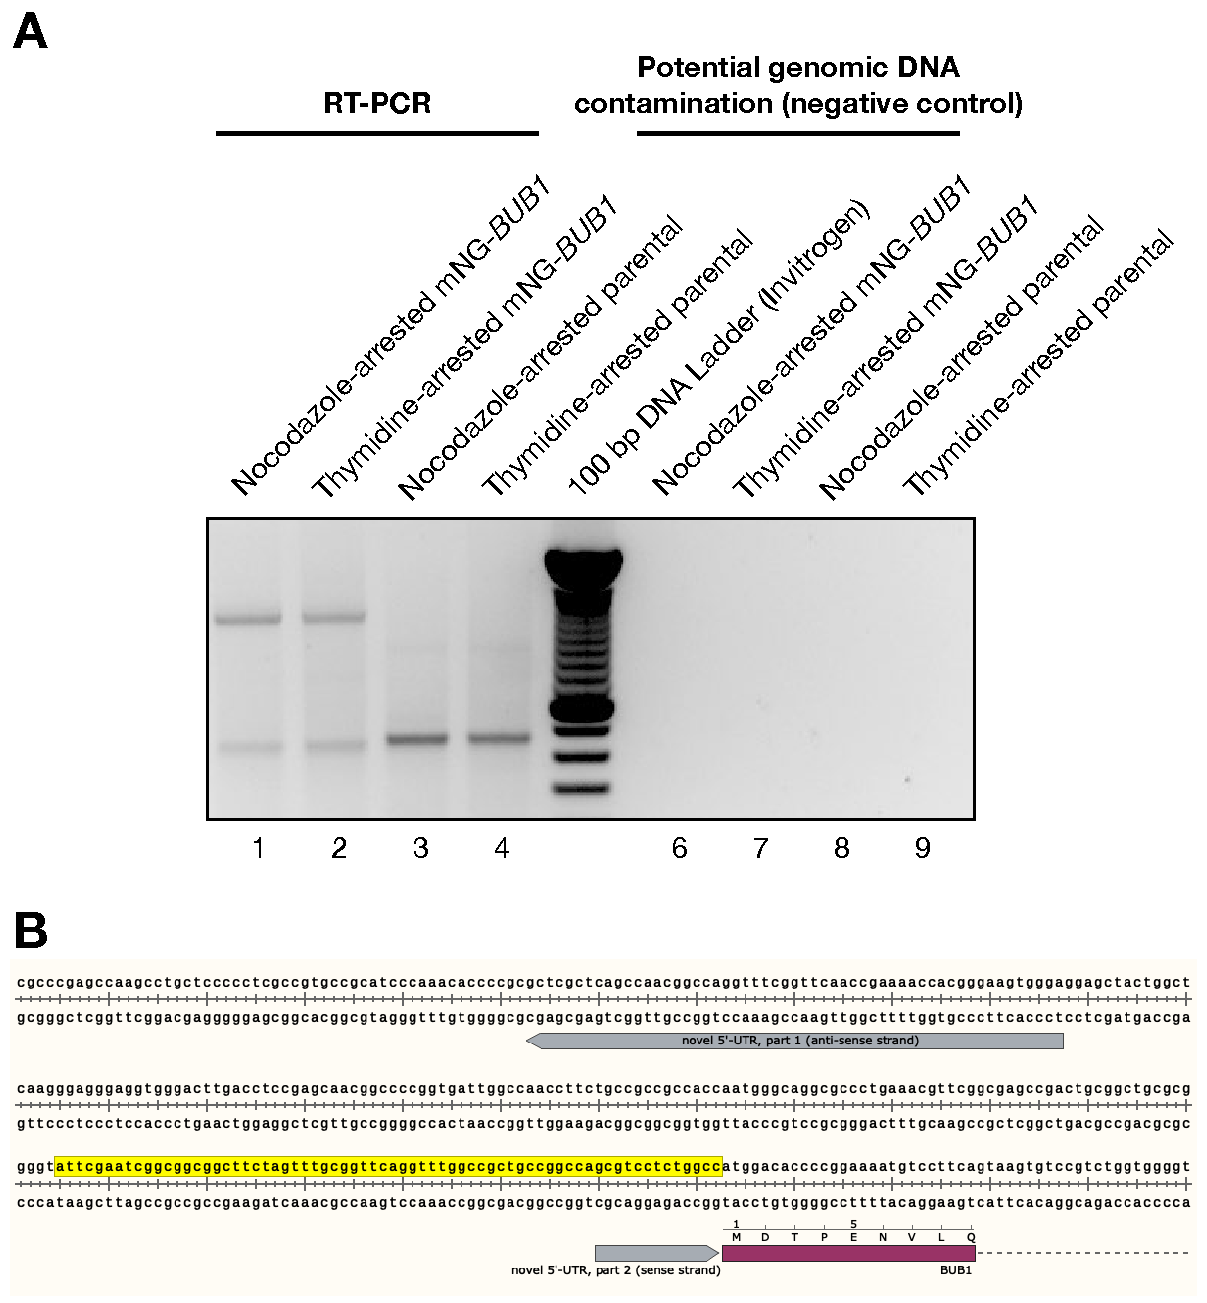
\includegraphics[width=\textwidth]{chapters/figures/5RACE.pdf}
    \phantomsubfiglabel{BUB1_5RACE} % subfigure A
    \phantomsubfiglabel{mNG-BUB1_5UTR_Seq} % subfigure B
    \caption{\textbf{5'-RACE identifies the 5'-UTR sequences of different \gene{Bub1} alleles in the genome-edited mNG-\gene{Bub1} cell line.}}
    \label{5RACE}
\end{figure}
\begin{figure} [t!]
    \noindent\justifying \textbf{(Caption of \myref{5RACE} continued from a previous page)} (A) 5'-RACE RT-PCR products using mitotic or G$_1$ total RNA extracts from  the mNG-\gene{Bub1} cells or the parental HeLa-A12 cells. The right four lanes used purified total RNAs directly as the PCR templates without the reverse transcription reaction, which served as negative controls for any remaining genomic DNA that could affect the interpretation of these results. (B) The 5'-UTR of wild-type \gene{Bub1} mRNA (highlighted in yellow) identified from the parental HeLa-A12 cells and the 5'-UTR of the novel \gene{Bub1} mRNA identified from the mNG-\gene{Bub1} cells that still translates into the wildtype \protein{Bub1} protein (the two-part gray arrows). The 5'-UTR of the wildtype \gene{Bub1} mRNA is composed of -68 to -1 of the sense strand. The 5'-UTR of the novel \gene{Bub1} mRNA is composed of -206 to -260 of the anti-sense strand followed by -13 to -1 of the sense strand, which indicates a possible chromosomal rearrangement event. The 5'-UTR of the mRNA transcribed from the mNG-\gene{Bub1} allele (corresponding to the upper bands of the first 2 lanes on the left) is the same as the 5'-UTR of the mRNA transcribed from the wildtype \gene{Bub1} allele in the parental HeLa-A12 cells, confirming that our \Latin{in situ} tagging does not affect the transcription start site (TSS) of \gene{Bub1}. Different clones may have slightly varied TSSs (data not shown). For reference, the PAM sequence used in the initial CRISPR-Cas9-mediated genome editing spans from -19 to -17 of the sense strand. The nucleotide coordinates are based on the reference sequence (NC\_000002.12, chromosome 2 of the GRCh38.p13 primary assembly).
\end{figure}

\section{The recruitment of \protein{Bub1} to signaling kinetochores had a major depletion effect on the cytosolic pool of \protein{Bub1}}

To test whether the cytosolic pools of SAC proteins were effectively diminished due to their recruitment to signaling kinetochores, we used fluorescence correlation spectroscopy (FCS) to quantify the abundance of \protein{Bub1} and \protein{BubR1} in cells treated with either MG132 (a proteasome inhibitor which arrests mitotic cells in the metaphase independently of the SAC) or nocodazole. In MG132-treated cells, SAC proteins are mostly in the cytosol but not recruited to the kinetochores. By comparing the cytosolic concentration of SAC proteins between cells treated with two different drugs, we can assess the depletion effect.
% needs citations

We estimated the cytosolic concentration of mNG-\protein{BubR1} and mNG-\protein{Bub1} in the corresponding MG132-treated HeLa-A12 cell line to be $(2.4 \pm 0.4) \times 10^2$ and $(1.0 \pm 0.25) \times 10^2$ nM, respectively (\myref{anti-mNG,FCS}). Importantly, we confirmed that the cytosolic concentration of \protein{Bub1} in nocodazole-treated cells was significantly lower than that in MG132-treated cells, indicating that the recruitment of \protein{Bub1} to signaling kinetochores diminished the cytosolic pool of \protein{Bub1}. This effect was not statistically significant for \protein{BubR1}. One explanation could be that the cellular concentration of \protein{BubR1} is higher than \protein{Bub1}. Given that \protein{BubR1} is mainly recruited to signaling kinetochores by heterodimerizing with \protein{Bub1} and that the stoichiometry is $1:1$ \Latin{in vitro} \cite{BubBiochem}, the depletion effect is naturally less prominent, especially when quantified by the auto-correlation at the 0-time lag ($G_0$, which is inversely proportional to the average number of freely diffusive fluorescent proteins/particles in the excitation volume; see \myref{FCSMethods}) derived from the FCS experiment.

% Total concentration of SAC proteins stay the same for Noc- and MG132-treated cells?

\section{The numbers of \protein{BubR1}, \protein{Bub1}, and \protein{Mad1} recruited per signaling kinetochore are inversely correlated with the total number of signaling kinetochores in the cell}

A natural outcome of the depletion effect partially demonstrated in the previous section is that the number of SAC proteins recruited per signaling kinetochore will be inversely correlated with the total number of signaling kinetochores in the cell. Indeed, our previous measurement in the budding yeast \cite{Aravamudhan2016} proved that it is the case. To validate this in our genome-edited HeLa-A12 cells, we first need to obtain mitotic cells containing distinctly different numbers of signaling kinetochores.

To obtain mitotic cells with nearly all kinetochores activating the SAC, we treated mitotic cells with \SI{330}{nM} nocodazole, a drug that destabilizes microtubules. These nocodazole-treated cells resemble normal mitotic cells at the start of the prometaphase.

To obtain mitotic cells with a much smaller number of signaling kinetochores, we treated mitotic cells with GSK923295, a \protein{Cenp-E} inhibitor that impairs chromosome alignment \cite{GSK923295}. In these cells, usually a variable but smaller number of chromosomes are stranded near the spindle poles (\myref{SACProteinKinetochoreRecruitment_Images}). We analyzed only those cells that contained ten or less than ten polar chromosomes. Kinetochores on these polar chromosomes are either unattached or laterally attached, which activate the SAC \cite{GSK923295LateralAttachmentEM, GSK923295MonastrolCotreatment}. These GSK923295-treated cells arguably (see discussions in \myref{Chapter3Discussions}) resemble normal mitotic cells near the end of the prometaphase.

\begin{figure} [b!]
    \centering
    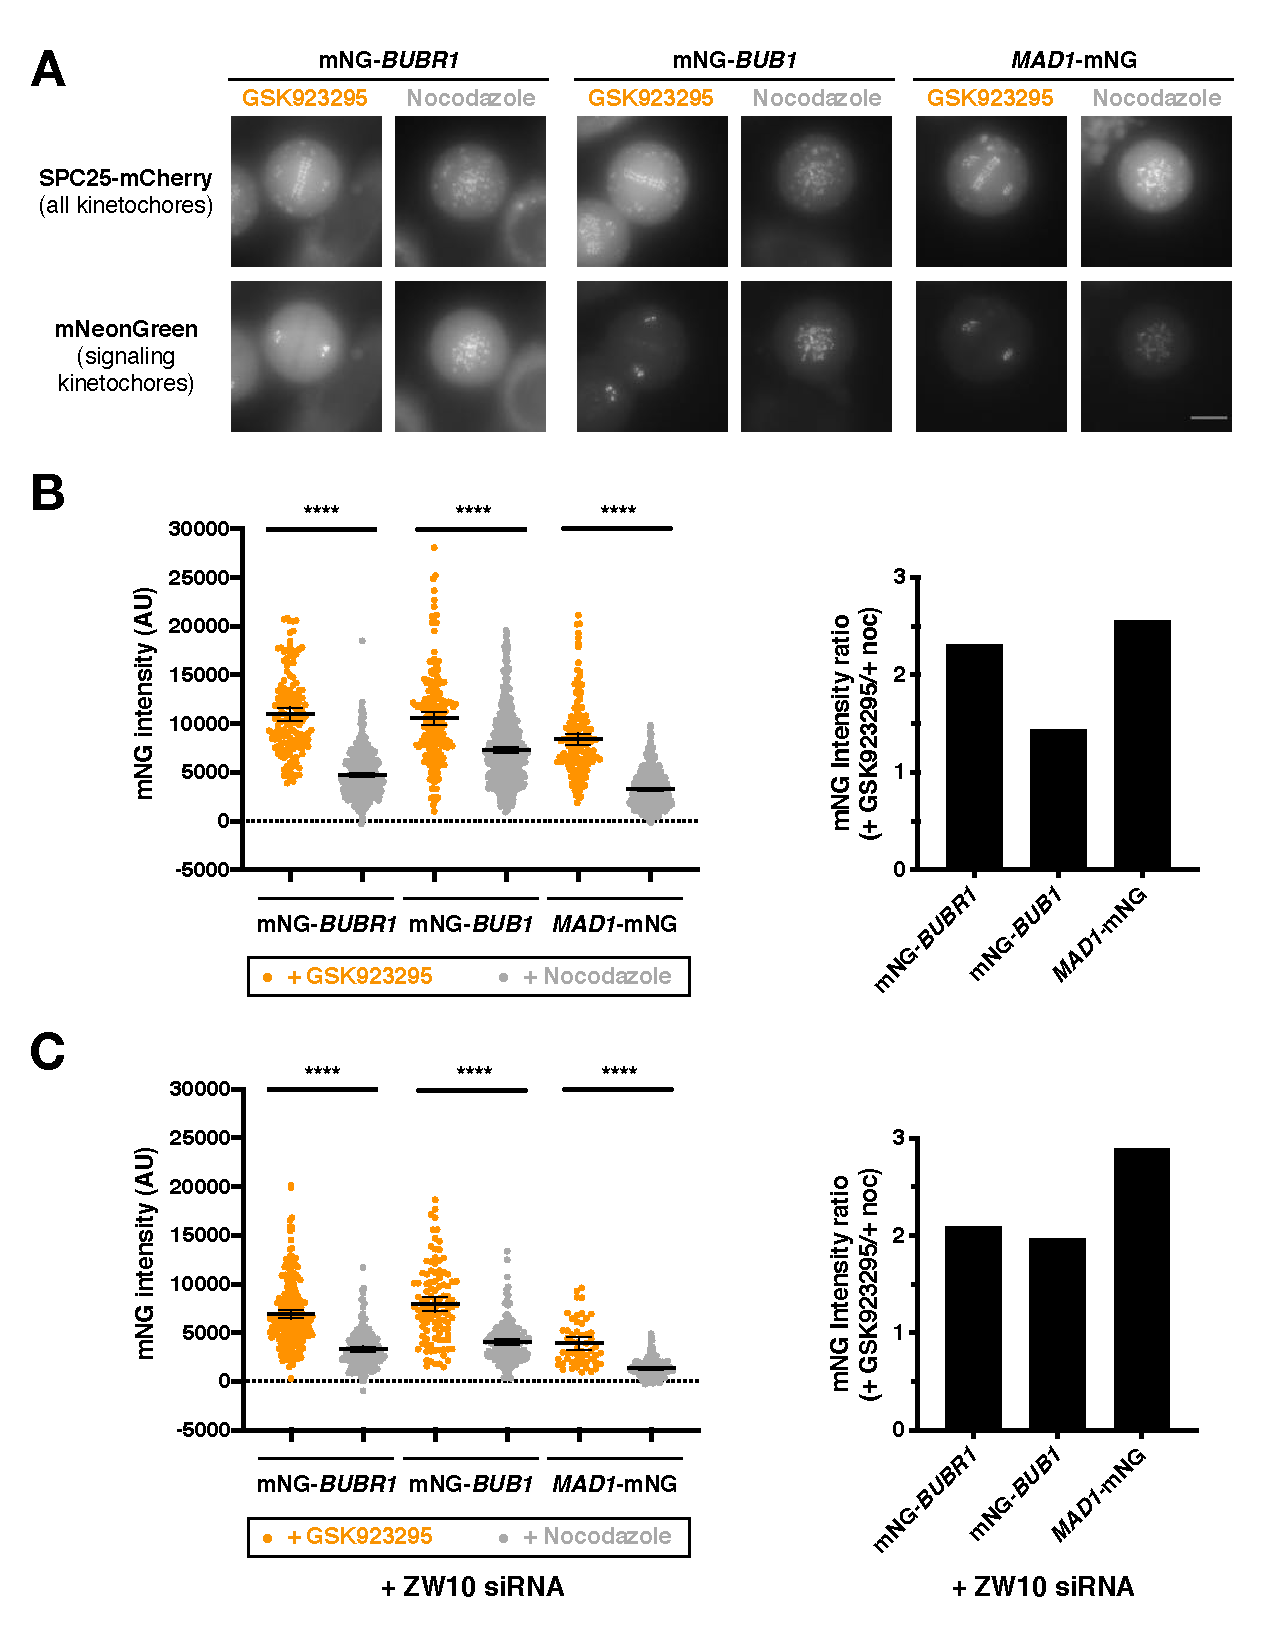
\includegraphics[width=0.95\textwidth]{chapters/figures/SACProteinKinetochoreRecruitment.pdf}
    \phantomsubfiglabel{SACProteinKinetochoreRecruitment_Images} % subfigure A
    \phantomsubfiglabel{SACProteinKinetochoreRecruitment_Quantification} % subfigure B
    \phantomsubfiglabel{siZW10SACProteinKinetochoreRecruitment_Quantification} % subfigure C
    \caption{\textbf{The numbers of \protein{BubR1}, \protein{Bub1}, and \protein{Mad1} recruited per signaling kinetochore are inversely correlated with the total number of signaling kinetochores in the cell.}}
    \label{SACProteinKinetochoreRecruitment}
\end{figure}
\begin{figure} [t!]
    \noindent\justifying \textbf{(Caption of \myref{SACProteinKinetochoreRecruitment} continued from a previous page)} \myref{SACProteinKinetochoreRecruitment_Quantification,siZW10SACProteinKinetochoreRecruitment_Quantification} were reproduced from one of my first-author manuscripts in preparation. Lauren Humphrey-Stark performed all imaging experiments and data analysis involved in this figure. (A) Representative micrographs showing cells from the three genome-edited HeLa-A12 cell lines treated with nocodazole or GSK923295. \protein{Spc25}-mCherry labeled all kinetochores \cite{Kukreja2020}. The coding sequence of \protein{Spc25}-mCherry was integrated into the genome of these HeLa-A12 cell lines immediately downstream of the constitutive \gene{EF1A} promoter (see \myref{Cre-lox}). Brightness and contrast have been adjusted but the LUT for each channel (row) is universal for different groups (column). Scale bar, \SI{10}{\micro m}. (B) Left panel: quantification of mNeonGreen signals at individual signaling kinetochores from experiments illustrated in (A). Each dot represents the measurement from one signaling kinetochore. Error bars represent 95\% confidence intervals of the mean. Results from at least two independent experiments are shown. Right panel: Pairwise ratios between the average mNeonGreen signals at individual signaling kinetochores of GSK923295-treated cells and nocodazole-treated cells in the left panel. (C) Similar to (B), except that all cells were additionally treated with a siRNA against \gene{ZW10}.
\end{figure}

In nocodazole-treated cells, the number of mNG-\protein{BubR1} and \protein{Mad1}-mNG proteins recruited per signaling kinetochore in nocodazole-treated cells was lower than that of mNG-\protein{Bub1} recruitment (\myref{SACProteinKinetochoreRecruitment_Quantification}). Importantly, \protein{BubR1}, \protein{Bub1}, and \protein{Mad1} recruitment per signaling kinetochore were all significantly increased when cells were treated with GSK923295 compared to nocodazole (\myref{SACProteinKinetochoreRecruitment_Quantification}). This confirms that the number of SAC proteins recruited per kinetochore is indeed inversely correlated with the number of signaling kinetochores in the cell.

In human cells, \protein{Mad1} is also recruited to the fibrous corona around a signaling kinetochore \cite{RZZ-MAD1vsBUB1-MAD1_2015, RZZ-MAD1vsBUB1-MAD1_2018}, which may contribute to the measurement in \myref{SACProteinKinetochoreRecruitment_Quantification} through widefield fluorescence microscopy. The corona is mainly composed of the ROD-Zwilch-ZW10-Spindly (RZZS) complex \cite{RZZS_Sacristan2018}. A previous study found conflicting dependency of the kinetochore localization of \protein{BubR1} on the RZZS complex in \Latin{Xenopus} extracts versus HeLa cells \cite{BUBR1_XenopusVSHeLa}. Another study observed that the kinetochore localization of \protein{BubR1} and \protein{Bub1} in the presence of \SI{660}{nM} nocodazole even increased when cells were treated with a siRNA against \gene{ROD} (see Figure 1E of \cite{siROD_Zhang2019}).

To dissect how much the core SAC pathway contributes to the recruitment of these SAC proteins at signaling kinetochores, we knocked down \gene{ZW10}, a subunit of the RZZS complex, by a siRNA against \gene{ZW10}. We then quantified the recruitment of the mNG-labeled SAC proteins to signaling kinetochores as before. Consistent with previous studies \cite{CENPELocalization-BUBR1,siROD_Zhang2019}, \protein{Mad1} recruitment was significantly lower in both GSK923295 and nocodazole-treated cells when the RZZS complex was knocked down (\myref{siZW10SACProteinKinetochoreRecruitment_Quantification}). The number of \protein{BubR1} and \protein{Bub1} molecules recruited per signaling kinetochore was also reduced, which deviates from previous studies. We hypothesized that unlike our \Latin{in situ} tagging, the immunofluorescence labeling used in the quantification of the kinetochore localization of \protein{BubR1} and \protein{Bub1} \cite{BUBR1_XenopusVSHeLa,siROD_Zhang2019} may be additionally affected by the accessibility of the antigen (\protein{BubR1} and \protein{Bub1}) to the corresponding antibody, which could be increased by the removal of the fibrous corona on the periphery of kinetochores. Importantly, the number of SAC proteins recruited per kinetochore was still inversely correlated with the number of signaling kinetochores in the cell.

\section{The chemical equilibrium between the activity of \protein{Mps1} and counteracting phosphatases at signaling kinetochore is the same in nocodazole- and GSK923295-treated HeLa-A12 cells}

The observed difference in the recruitment of SAC proteins on a per kinetochore basis in nocodazole- and GSK923295-treated cells may be alternatively attributed to different degrees of phosphorylation of MELT motifs. This could be an indirect result of the various effect of different drugs on the kinetochore-microtubule attachment (see Figure 3f of \cite{Rheostat}). It may also be due to previously uncharacterized regulations of different drugs imposed on the activity of kinases and counteracting phosphatases at the kinetochore directly.

To test this alternative hypothesis in the HeLa-A12 cell line, we probed the equilibrium between the activity of kinases (mainly \protein{Mps1}) and counteracting phosphatases at the kinetochore (henceforth referred to as ``\protein{Mps1}'s activity'' for simplicity) using a similar phosphorylation sensor (MPS1sen-KT; see \myref{MPS1sen-KT_Scheme}) to the one developed in a previous study \cite{MPS1senor}. The original idea of this F{\"{o}}rster resonance energy transfer (FRET) sensor design was first proposed in \cite{FHA2BasedFRETSensorOriginalStudy}. The chemical equilibrium between the activity of kinases and counteracting phosphatases determines the phosphorylation level of the substrate. If the substrate has a higher level of phosphorylation, FHA2 (the phospho-threonine binding domain from the yeast protein Rad53p) will have a higher affinity to bind to the substrate, thereby distancing the donor and the acceptor better and resulting in lower FRET efficiency. The expression cassette of the recombinant sensor is under the regulation of TRE and stably integrated into the genome of HeLa-A12 cells via Cre-\bacterialgene{lox} RMCE. The acceptor and the donor have a fixed $1 : 1$ stoichiometry by design and the recombinant sensor was mostly intact in the cell (with no major partial degradation species like mScarlet-I-\protein{Spc24} alone; see the immunoblot in \myref{MPS1sen-KT_Images}). Therefore, the ratio between the green channel readout and the raw FRET channel readout (even without corrections for the cross-excitation of the acceptor and the bleed-through of donor fluorescence) can be employed as a normalized measurement of the FRET efficiency (see \myref{FRETMetricTheory}) and serve as an indicator of \protein{Mps1}'s activity.

\begin{figure} [b!]
    \centering
    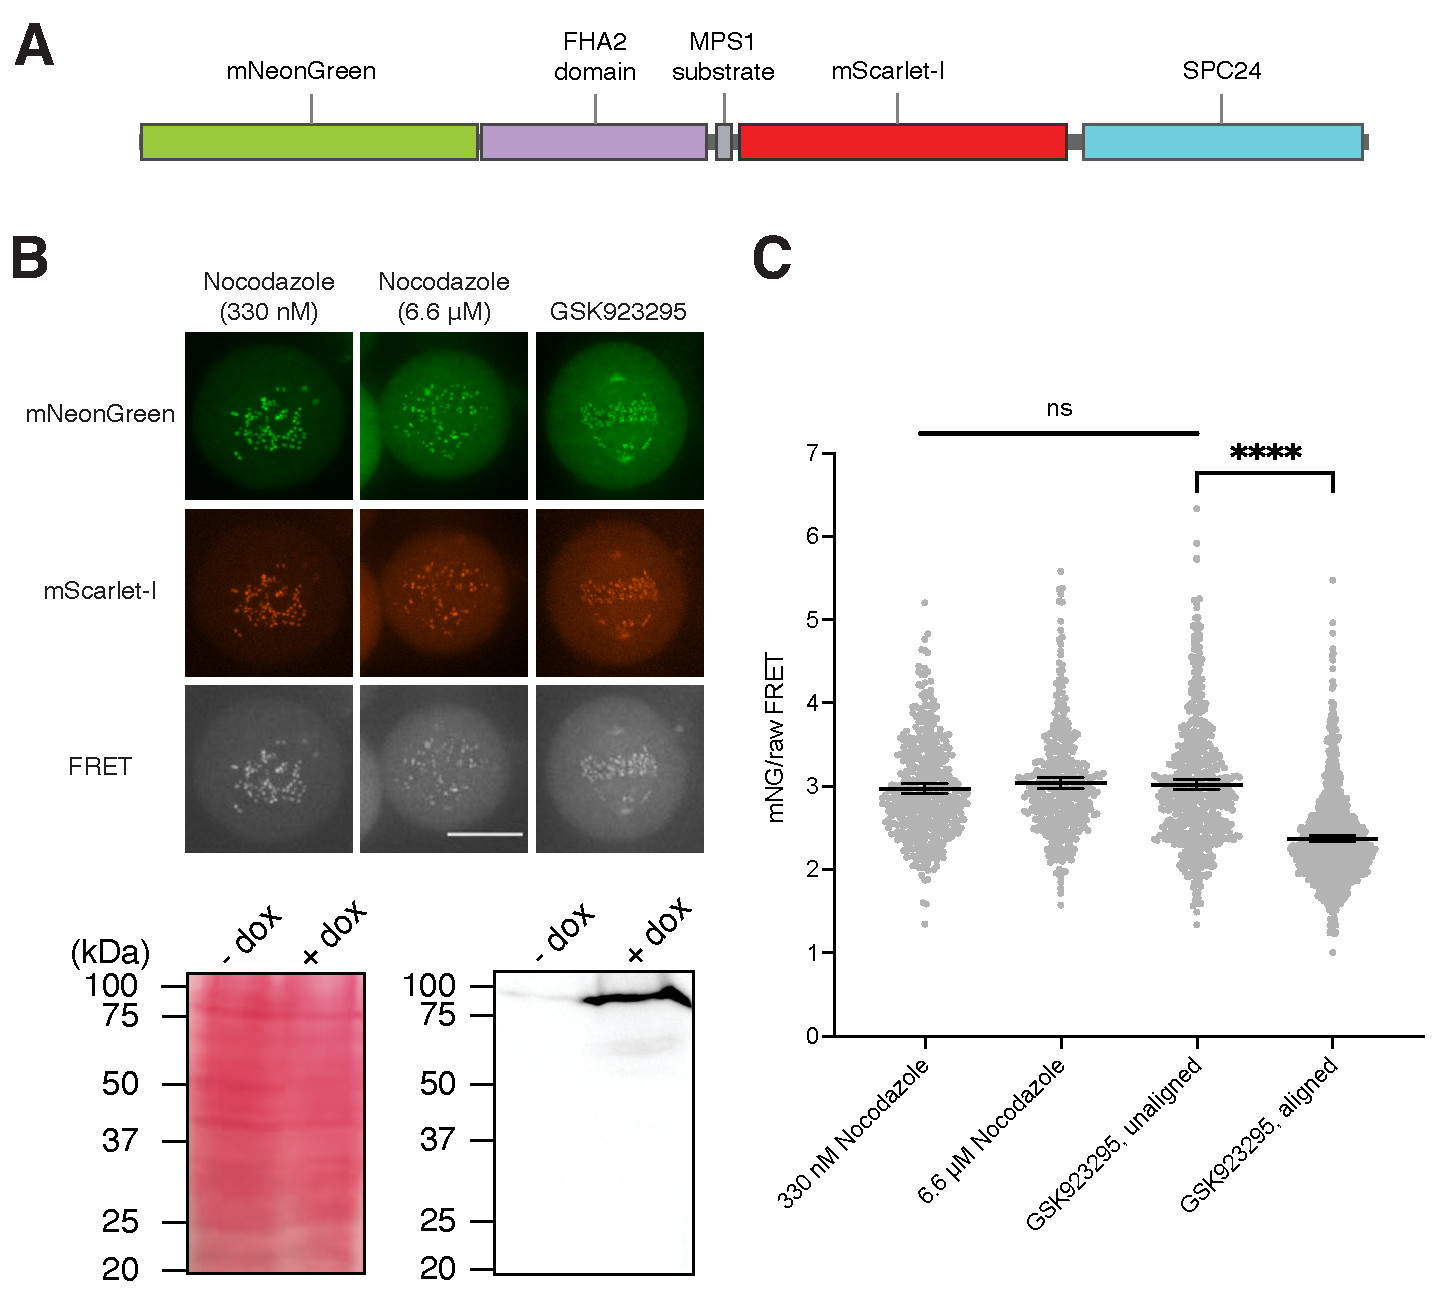
\includegraphics[width=\textwidth]{chapters/figures/MPS1sen-KT.pdf}
    \phantomsubfiglabel{MPS1sen-KT_Scheme} % subfigure A
    \phantomsubfiglabel{MPS1sen-KT_Images} % subfigure B
    \phantomsubfiglabel{MPS1sen-KT_FRETMetric} % subfigure C
    \caption{\textbf{No difference in the \protein{Mps1}-phosphatases equilibrium at signaling kinetochores was detected in HeLa A12 when cells were treated with different drugs at various concentrations.}}
    \label{MPS1sen-KT}
\end{figure}
\begin{figure} [t!]
    \noindent\justifying \textbf{(Caption of \myref{MPS1sen-KT} continued from a previous page)} (A) The design scheme of MPS1sen-KT. The \protein{Mps1} substrate sequence is \Peptide{LLEDGTLAINW}.
    The only difference between our version of the MPS1sen-KT and the original design \cite{MPS1senor} is that we used mNeonGreen/mScarlet-I as the acceptor/donor combination, which suits our confocal microscopy setup. (B) Top panel: representative images of cells expressing MPS1sen-KT. MPS1sen-KT was recruited to both unaligned signaling kinetochores (in Nocodazole- and GSK923295-treated cells) and non-signaling kinetochores aligned at metaphase plates (in GSK923295-treated cells) via its C-terminal \protein{Spc24} module. Brightness and contrast have been adjusted but the LUT for each channel (row) is universal for different groups (column). Scale bar, \SI{10}{\micro m}. Bottom panel: using an antibody against DsRed2 (which can detect many RFPs including mScarlet-I), we confirmed that MPS1sen-KT (with a theoretical molecular weight of \SI{97.2}{kDa}) can be induced by doxycycline to express as a full-length protein with negligible partial degradation or cleavage products in the RMCE HeLa-A12 cells (right blot). The Ponceau S staining of the same blot before blocking (left blot) served as the loading and transfer control. (C) A summary of a normalized FRET metric (mNeonGreen signal/FRET signal) in HeLa A12 cells treated with different drugs at various concentrations. Each gray dot represents a single kinetochore measurement. Data were compiled from at least two independent experiments (with more than 40 cells and 400 kinetochores in each group). Mean values $\pm 95\%$ confidence intervals are overlaid. Data from cells treated with \SI{45}{nM}, \SI{90}{nM}, and \SI{200}{nM} GSK923295 were pooled together (they have no significant difference from one another) to simplify the presentation. The Welch's ANOVA test [$W(\text{DF}n, \text{DF}d) = 1.339 (2.000, 917.0)$, $P = 0.2626$] was performed for the first 3 columns (signaling kinetochores). The unpaired $t$-test with Welch's correction ($P < 0.0001$) was performed to compare non-signaling kinetochores aligned at metaphase plates with unaligned signaling kinetochores in GSK923295-treated cells. Statistical tests were done in Prism 9.
\end{figure}

We confirmed that MPS1sen-KT recruited to unaligned signaling kinetochores in both nocodazole- and GSK923295-treated cells had lower FRET efficiencies (higher \protein{Mps1}'s activity) compared to MPS1sen-KT recruited to non-signaling kinetochores aligned at metaphase plates in GSK923295-treated cells (\myref{MPS1sen-KT_FRETMetric}), consistent with the previous study \cite{MPS1senor}. However, in contrast to \cite{MPS1senor}, we did not observe any difference in \protein{Mps1}'s activity at unaligned signaling kinetochores in nocodazole- versus GSK923295-treated cells. This was irrelevant to the concentrations of respective drugs and the reason for the conflicting observations may be explained by cell line-specific effects. As far as the HeLa-A12 cell line is concerned, the difference in the numbers of SAC proteins recruited per signaling kinetochore in nocodazole- and GSK923295-treated cells should be mainly attributed to the difference in the total number of signaling kinetochores, which all compete for the limited pools of SAC proteins in the cell based on the law of mass action.

% It has been reported previously that the average localization levels of endogenously tagged HA-mCherry-\protein{Bub1} to signaling kinetochores in a CRISPR-Cas9-edited HeLa cell line treated with either \SI{250}{nM} of GSK923295 or \SI{6.6}{\micro M} of nocodazole were not significantly different \cite{MPS1senor}. One possible explanation is that the much higher concentration of nocodazole in the aforementioned study may contribute to a more complete breakdown of spindles and a higher number of phosphorylated MELT motifs, while the higher concentration of GSK923295 and the lack of filtering of cells based on the total number of unaligned chromosomes could mean more signaling kinetochores in GSK923295-treated cells.

%This observation contrasts with the previous report that the average localization levels of endogenously tagged HA-mCherry-Bub1 to signaling kinetochores in a CRISPR-Cas9-edited HeLa cell line treated with either 250 nM of GSK923295 or 6.6 μM of nocodazole were not significantly different (Kuijt et al., 2020). One possible explanation is that the much higher concentration of nocodazole in the aforementioned study may contribute to a more complete breakdown of spindles and a higher degree of phosphorylation of MELT motifs, while the lack of filtering of GSK923295-treated cells based on the number of unaligned chromosomes would lead to similar average numbers of signaling kinetochores in the Nocodazole- and GSK923295-treated cells. We also cannot rule out the possibility that the differences reflect different Bub1 expression levels or kinase/phosphatase activities in the HeLa cell lines used.

\section{Recruitment of \protein{BubR1} by \protein{Bub1} \Latin{per se} contributes to the activity of the kinetochore-based SAC signaling}
\label{per_se}

Finally, we wanted to prove that the co-localization of multiple SAC proteins on the same \protein{Knl1} scaffold cooperatively boosts the kinetochore-based SAC signaling activity. Unfortunately, testing this non-linearity \Latin{in vivo} is currently beyond our capability considering the technical challenge to quantify the real-time signaling activity for each signaling kinetochore. As a compromise, we set out to prove that the enrichment of SAC proteins at kinetochores strengthens the SAC signaling.

Previous studies showed that \protein{BubR1} is mainly recruited to signaling kinetochores by heterodimerizing with \protein{Bub1} \cite{BubBiochem,BubR1TwoPools}. \protein{Bub1} is an important hub protein that binds to other SAC proteins (like \protein{Cdc20} and \protein{Mad1} which coordinately promote the formation of the \protein{Cdc20}-\protein{Mad2} heterodimer \Latin{in vitro} and in \Latin{Caenorhabditis elegans} \cite{BUB1-CDC20-MAD1,Tripartite}). We reasoned that \protein{BubR1}'s recruitment to signaling kinetochores by \protein{Bub1} may cause the local enrichment of \protein{BubR1} near where the \protein{Cdc20}-\protein{Mad2} dimer is formed and thereby facilitate the assembly of the MCC better than cytosolic free \protein{BubR1} does. Our eSAC activator-based assay (using truncations of \protein{Bub1} as the scaffold protein instead of the recombinant \protein{Knl1} phosphodomain in \myref{chpt2}) showed that the recombinant \protein{Bub1} which can bind \protein{BubR1} promotes the SAC signaling activity better than the recombinant \protein{Bub1} which is unable to bind \protein{BubR1} does (manuscript in preparation). However, other previous studies show that either the deletion of the heterodimerization domain of \protein{Bub1} (in an in vitro assay \cite{BUB1-CDC20-MAD1}) or the mutation of the GLEBS domain of kinetochore-tethered \protein{Bub1} \cite{MIS12-BUB1-E252K}, both of which abolished the heterodimerization between \protein{Bub1} and \protein{BubR1}, does not affect the SAC signaling activity. Moreover, two previous \protein{BubR1} knockdown-rescue experiments in nocodazole-treated cells published by different research groups demonstrated that \protein{BubR1}'s recruitment to signaling kinetochores by \protein{Bub1} counter-intuitively shortens the duration of the mitotic arrest \cite{BubR1TwoPools,BubBiochem}. Even though the two studies deleted different segments of \protein{BubR1}'s heterodimerization domain which mediates \protein{BubR1}'s interaction with \protein{Bub1} (a.a 440-460 \cite{BubR1TwoPools}, henceforth referred to as ``HD\textsuperscript{short}'', versus a.a. \textDelta{}432-484 \cite{BubBiochem}, henceforth referred to as ``HD'') and used different concentrations (\SI{\sim100}{nM} in \cite{BubR1TwoPools} versus \SI{50}{nM} in \cite{BubBiochem}) of nocodazole to induce signaling kinetochores, their basic observations were nonetheless consistent. We also did a similar knockdown-rescue experiment in GSK923295-treated cells comparing the SAC signaling activity of wildtype \protein{BubR1} and \protein{BubR1}(\textDelta{}HD\textsuperscript{short}), whose results were also consistent with these two studies (\myref{OldBUBR1Rescue}). These conflicting pieces of evidence inspired us to examine the matter more carefully.
% which might have resulted in the observation of different levels of heterodimerization domain-truncated \protein{BubR1} remaining at signaling kinetochores.
% We hypothesize that this pool of BUBR1 comes into spatial proximity with other MCC components and thereby facilitates the MCC assembly.

We noted that first, there was no rigorous control over the expression level of the ectopic recombinant \protein{BubR1} to match the physiological expression of endogenous \protein{BubR1} in these two studies.

Second, the concentrations of nocodazole used in these two studies allowed the existence of some spindle microtubules \cite{100nMNoc}. However, PP2A's recruitment by \protein{BubR1}'s kinetochore attachment regulatory domain (KARD) to signaling kinetochores is known to contribute to the silencing of the SAC either directly (by dephosphorylating the MELT motif \cite{PP2ADephosphorylatesKNL1} or \protein{Bub1} \cite{PP2ADephosphorylatesBUB1}) or indirectly (by stabilizing the kinetochore-microtubule attachment \cite{BUBR1_KT-MT, Suijkerbuijk2012, BUBR1-L669A+I672A, PP2A-B56-BUBR1ChromosomeCongression_Xu2013} or promoting PP1's recruitment \cite{PP2A-B56}). PP2A's recruitment to signaling kinetochores might not be completely canceled by \protein{BubR1}(\textDelta{}HD)'s defective interaction with B56 \cite{BubBiochem}, RNA interference against B56's (due to probable incomplete knock-down), or KARD mutations (\cite{BubR1TwoPools}, which eliminated the binding of the B56\textalpha{} isoform \cite{BUBR1-L669A+I672A}).

Third, although the depletion of \protein{BubR1} does not affect the localization of \protein{Cenp-E} at signaling kinetochores in HeLa cells \cite{CENPELocalization-BUBR1}, the activity of kinetochore-localized \protein{Cenp-E} (to facilitate the transition of the kinetochore-microtubule attachment from lateral to end-on) is arguably affected by the loss of interaction with \protein{BubR1} \cite{CENPEActivity-BUBR1} when cells are rescued by heterodimerization domain-truncated \protein{BubR1}, which may thereby affect chromosome congression. % CENP-E binds to PP1 and Aurora kinases can dynamically regulate this interaction to promote chromosome alignment (Kim et al., 2010). 

Therefore, we designed and performed a new \protein{BubR1} knockdown-rescue experiment. Here, the SAC signaling activity of \protein{BubR1}(\textDelta{}KARD) and \protein{BubR1}(\textDelta{}KARD, \textDelta{}HD) was compared (\myref{RecombinantBUBR1Diagram}). The truncation of KARD (a.a. 665-682) abolishes the binding of B56\textalpha{} \cite{Suijkerbuijk2012} and likely other isoforms of B56 onto \protein{BubR1} as well \cite{B56-SLiM, PP2A-B56-BUBR1Structure}, which allow us to dissect whether the recruitment of \protein{BubR1} to the signaling kinetochore \Latin{per se} contributes to the SAC activity. Additionally, mNG-\protein{BubR1}(\textDelta{}HD, \textDelta{}KARD) lacks the heterodimerization domain (HD). We imaged our genome-edited mNG-\gene{BubR1} HeLa-A12 cell line (treated with the AllStars negative control siRNA) at the same time to serve as a reference for the endogenous expression of \protein{BubR1} (first column, \myref{NewBUBR1Rescue}). Only mitotic cells having $0.5\times$ -- $2\times$ the average mNeonGreen intensity of mNG-\gene{BubR1} HeLa-A12 cells during mitosis were included in the analysis (noted that only about half of endogenous \protein{BubR1} proteins are tagged in the CRISPR-Cas9-edited cell line).

Just like what was shown in \cite{BubBiochem}, mNG-\protein{BubR1}(\textDelta{}HD, \textDelta{}KARD) had minimal localization at signaling kinetochores  (\myref{BUBR1del432-484KTLocalization}). The mitotic arrest was induced by treatment with \SI{25}{nM} of nocodazole \cite{25nMNoc} after thymidine release, where unattached kinetochores can be observed while metaphase plates remain largely intact (\myref{BUBR1del432-484KTLocalization}).

\begin{figure} [b!]
    \centering
    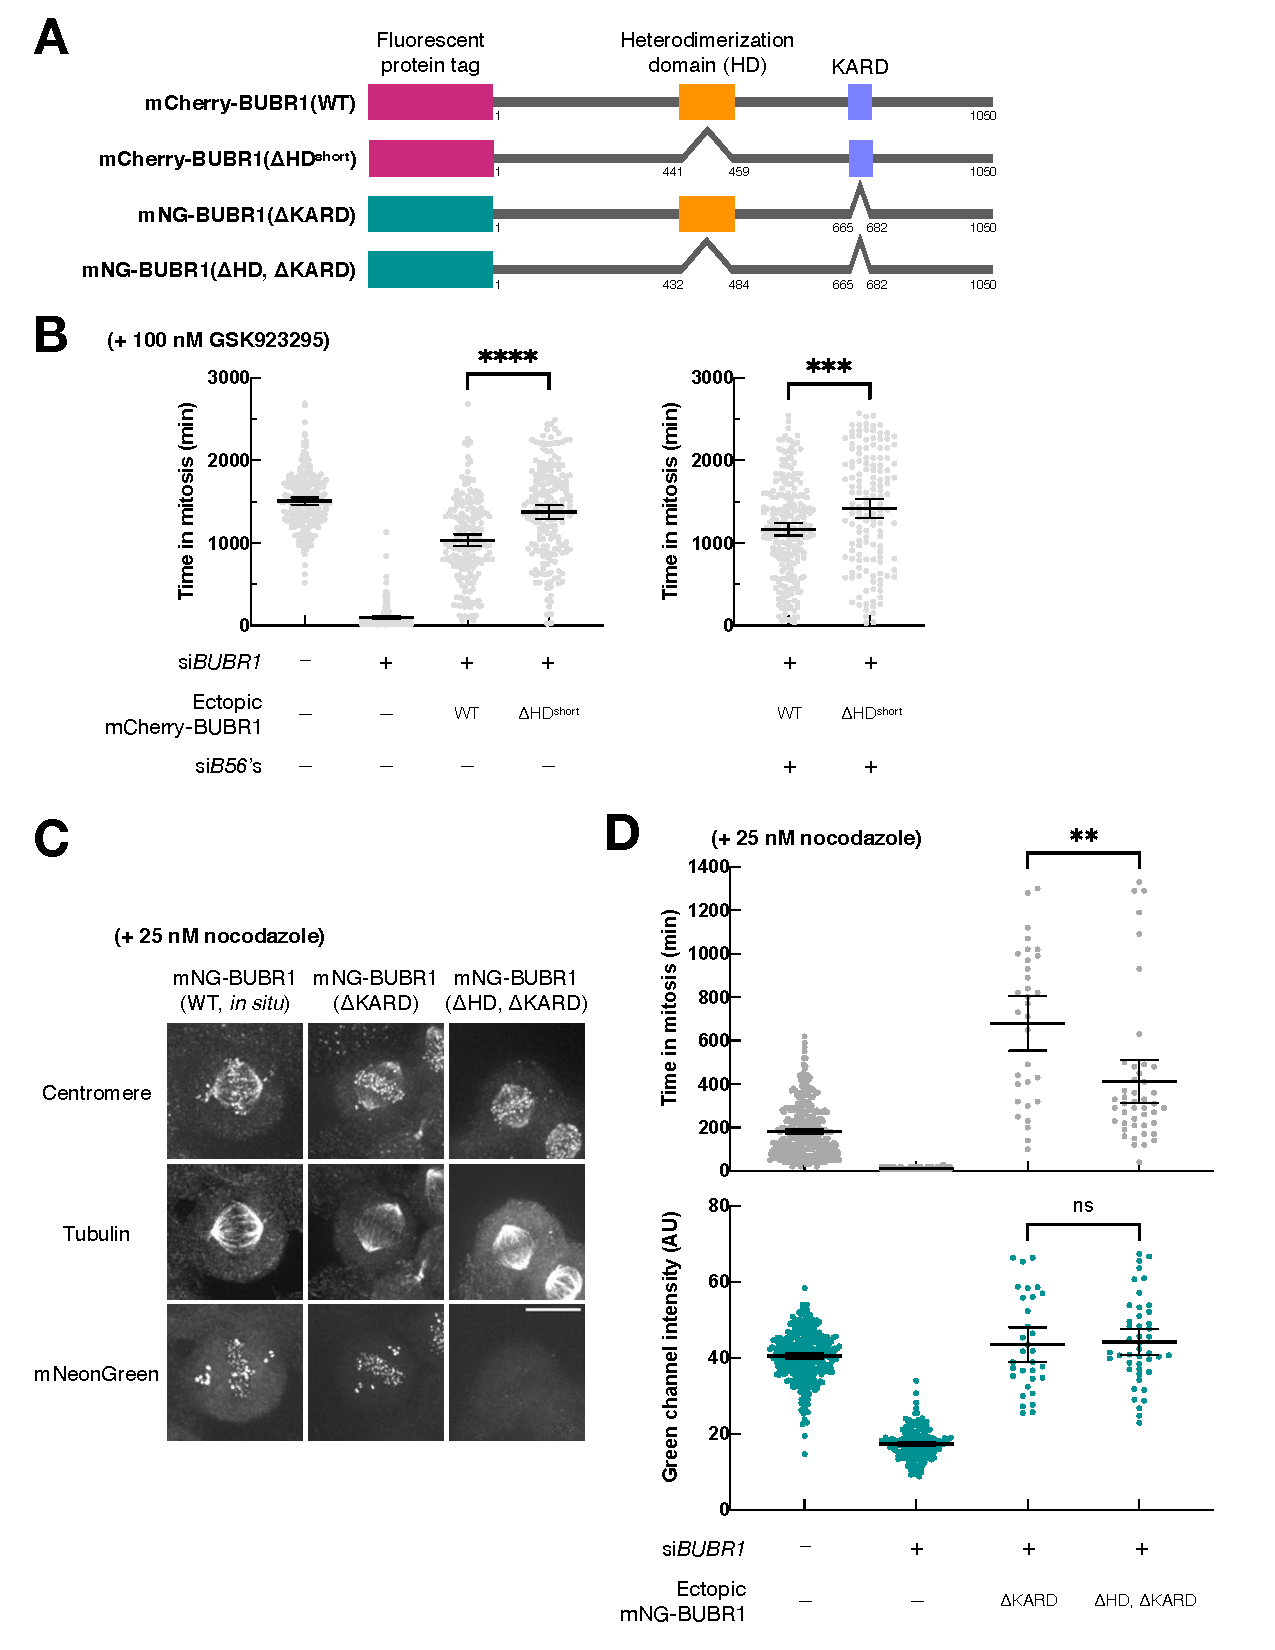
\includegraphics[width=\textwidth]{chapters/figures/RescueExperiment.pdf}
    \phantomsubfiglabel{RecombinantBUBR1Diagram} % subfigure A
    \phantomsubfiglabel{OldBUBR1Rescue} % subfigure B
    \phantomsubfiglabel{BUBR1del432-484KTLocalization} % subfigure C
    \phantomsubfiglabel{NewBUBR1Rescue} % subfigure D
    \caption{\textbf{Recruitment of \protein{BubR1} by \protein{Bub1} to signaling kinetochores \Latin{per se} contributes to the SAC signaling activity.}}
    \label{RescueExperiment}
\end{figure}
\begin{figure} [t!]
  \noindent\justifying \textbf{(Caption of \myref{RescueExperiment} continued from a previous page)} \textbf{(A)} Diagrams (not to scale) of all ectopic recombinant BUBR1's used in experiments associated with \myref{OldBUBR1Rescue,BUBR1del432-484KTLocalization,NewBUBR1Rescue}. \textbf{(B)} A \gene{BubR1} knockdown-rescue experiment with mCherry-\protein{BubR1} or mCherry-\protein{BubR1}(\textDelta{}HD\textsuperscript{short}) (with an HD truncation from \cite{BubR1TwoPools}). \cite{BubR1TwoPools} uses a shorter HD truncation compared to \cite{BubBiochem}. Therefore, it is denoted as \textDelta{}HD\textsuperscript{short} here. We used \SI{100}{nM} GSK923295 to activate the SAC signaling, which is different from both \cite{BubR1TwoPools} (\SI{100}{nM} nocodazole) and \cite{BubBiochem} (\SI{50}{nM} nocodazole). Cells rescued with mCherry-\protein{BubR1} consistently have a lower SAC signaling activity than cells rescued with mCherry-\protein{BubR1}(\textDelta{}HD\textsuperscript{short}), no matter whether B56's were knocked down. Cells treated with si\gene{BubR1} and rescued with mCherry-\protein{BubR1} had a lower SAC signaling activity than parental cells treated with the AllStars negative control siRNA, probably due to the lack of control over the expression of the ectopic mCherry-\protein{BubR1}. Each dot represents a cell, with more than 140 cells in each group. The mean value $\pm$ the 95\% confidence interval of each group is overlaid. Unpaired $t$-tests with Welch's correction were performed in Prism 9. Frank Ferrari also contributed to the data analysis here. \textbf{(C)} Confocal immunofluorescence micrographs (by Dr. Ajit Joglekar) showed that \SI{25}{nM} nocodazole impaired the congression of a few chromosomes (which activated the SAC) in both genome-edited mNG-\gene{BubR1} HeLa-A12 cells (the first column) and the RMCE HeLa-A12 cells (the second and the third columns). In the second and the third columns, the RMCE HeLa-A12 cells were treated with si\gene{BubR1} and \SI{0.5}{\micro g/mL} of doxycycline to induce the ectopic expression of indicated mN-\protein{BubR1} variants. Ectopically expressed mNG-\protein{BubR1}(\textDelta{}HD, \textDelta{}KARD) could not be detected at kinetochores (the third columns). Maximum $z$-projections of representative cells were shown for each condition (column) and channel (row). The LUTs for the mNeonGreen channel are the same across different conditions. Scale bar, \SI{10}{\micro m}. \textbf{(D)} A \gene{BubR1} knockdown-rescue experiment with mNG-\protein{BubR1}(\textDelta{KARD}) or mNG-\protein{BubR1}(\textDelta{}HD, \textDelta{}KARD) (with an HD truncation from \cite{BubBiochem}). Top panel: the duration of mitosis of individual cells treated with \SI{25}{nM} nocodazole. Bottom panel: the average cytosolic mNeonGreen signal from the same cells right after the NEBD. In the heterozygous, genome-edited mNG-\gene{BubR1} HeLa-A12 cells (first two columns), both the wildtype allele and the edited mNG-\gene{BubR1} allele are susceptible to si\gene{BubR1}. In the RMCE HeLa-A12 cells (last two columns), ectopically expressed mN-\protein{BubR1} variants are resistant to si\gene{BubR1}. Each dot represents a cell, with more than 30 cells in each group. Results are representative of two independent experiments. The mean value $\pm$ the 95\% confidence interval of each group is overlaid. Unpaired $t$-tests with Welch's correction were performed in Prism 9.
\end{figure}

Our knockdown of \gene{BubR1} was sufficient to almost completely abolish the SAC signaling (first two columns, \myref{NewBUBR1Rescue}). mNG-\protein{BubR1}(\textDelta{}KARD)-rescued cells take longer in mitosis than the control group (the third column versus the first column, \myref{NewBUBR1Rescue}), which is consistent with previous studies \cite{PP2A-B56, BUBR1-L669A+I672A}. Most importantly, our new data showed that mNG-\protein{BubR1}(\textDelta{}KARD)-rescued cells had a higher SAC signaling activity than mNG-\protein{BubR1}(\textDelta{}HD, \textDelta{}KARD)-rescued cells did (\myref{NewBUBR1Rescue}), directly supporting that the recruitment of \protein{BubR1} \Latin{per se} contributes to the activity of the kinetochore-based SAC signaling.

\section{Discussions}
\label{Chapter3Discussions}

In this chapter, we demonstrated that the competition among a large number of signaling kinetochores can effectively diminish freely diffusive SAC proteins in the cytosol. This, instead of a potential shift in the degree of phosphorylation of MELT motifs, presumably explains why the numbers of SAC proteins recruited per signaling kinetochore are inversely correlated with the total number of signaling kinetochores in the cell. Using the recruitment of \protein{BubR1} by \protein{Bub1} as an example, we showed that the co-localization of multiple SAC proteins on the same \protein{Knl1} scaffold likely strengthens the SAC signaling activity. Even though we did not rigorously prove that the cooperativity among multiple SAC proteins on the same \protein{Knl1} scaffold boosts the kinetochore-based SAC signaling activity non-linearly, all data presented in this chapter supported the model in \myref{ProzoneEffectModel}.

By knocking down \gene{ZW10}, we dissected the contribution of the core SAC pathway to the kinetochore localization of SAC proteins. However, it should be noted that \protein{Mad1} may also be recruited to signaling kinetochores by the kinetochore protein \protein{Cep57} \cite{MIS12-CEP57-MAD1-MAD2}. Further studies are needed to clarify whether the \protein{Cep57} pathway, the corona pathway, and the \protein{Knl1}-\protein{Bub1} (core SAC) pathway of \protein{Mad1} recruitment work cooperatively or independently.

The architecture of human kinetochores is proposed to resemble a Velcro-like interface for microtubule binding \cite{Velcro}. This ``lawn model'' proposes that the human kinetochore behaves like a network of adaptable attachment sites for an average number of about 17 microtubules in the metaphase \cite{Wendell1993, Zaytsev2014, Zaytsev2015, Kukreja2020}. The dynamic and stochastic establishment of kinetochore-microtubule attachment influences the localization of SAC protein and the dynein-dependent stripping of the corona \cite{SACSilencing_Etemad2019, SACSilencing_Kuhn2019, CENP-FLimitsStripping}. We envision that at the beginning of the prometaphase, all signaling kinetochores in a human cell are fully unattached. As the cell progress normally through the prometaphase, kinetochores gradually and independently establish end-on attachment to spindle microtubules. When we take a snapshot of a human cell near the end of the prometaphase, instead of one completely unattached kinetochores and 91 fully attached kinetochores that have already completely silenced their local SAC signaling activity, there may be three minimally attached kinetochores and 89 mostly attached kinetochores that are still in the process of stripping the corona and silencing the local SAC signaling activity. It remains to be seen whether (or how) the idea of dynamic regulation of the SAC signaling activity per kinetochore based on the total number of signaling kinetochores applies to this physiological scenario. % our quantification of the localization of SAC proteins to signaling kinetochores was performed in drug-arrested mitotic cells.

% The potentially reduced \protein{Cenp-E} activity at the kinetochore in mNG-\protein{BubR1}(\textDelta{}HD, \textDelta{}KARD)-rescued cells should only result in an increased SAC response, compared to mNG-\protein{BubR1}(\textDelta{}KARD)-rescued cells.
\protein{BubR1} interacts with the kinase \protein{Plk1}, a key regulator throughout mitosis \cite{BUBR1-PLK1}. mNG-\protein{BubR1}(\textDelta{}KARD) may still recruit \protein{Plk1} to signaling kinetochores, while mNG-\protein{BubR1}(\textDelta{}HD, \textDelta{}KARD) (which itself minimally localized to signaling kinetochores) can not. Although depletion of \protein{BubR1} only results in a marginal reduction of \protein{Plk1} at signaling kinetochores \cite{CENPU+BUB1-PLK1}, it remains to be examined how much the discrepancy in the localization of \protein{Plk1} contributes to the SAC signaling activity in the knockdown-rescue experiment of \protein{BubR1}.

In our manuscript, Soubhagyalaxmi Jema further showed that an increased expression of \protein{Bub1} enhanced the recruitment of \protein{BubR1} to signaling kinetochores and the SAC signaling activity. These observations demonstrated that the SAC signaling activity is partially limited by the low expression level of \protein{Bub1} in HeLa-A12 cells. We hypothesized that this could be the result of a compromise among various sources of selection pressure. Like \protein{BubR1}, whose recruitment to signaling kinetochores improves the SAC signaling activity and promotes chromosome congression, \protein{Bub1} also has multiple functions (for example, in telomere replication \cite{BUB3-BUB1_TelomereReplication} and the correction of erroneous kinetochore-microtubule attachment \cite{BUB1_pH2A_AuroraB}). The MCC is even involved in the clathrin-mediated endocytosis of insulin receptors \cite{MCC_IREndocytosis, Choi2019}. How these functions of SAC proteins interact and integrate is a fascinating topic that may lead to exciting discoveries. % (for example, between the sensitivity of the SAC to detect a small number of unattached kinetochores and the responsiveness of the SAC to silence once all chromosomes establish proper bipolar attachment and are aligned at the metaphase plate \cite{eSAC})

\section{Materials and Methods}
For methods of cell culture and Cre-\bacterialgene{lox} RMCE, see \myref{CellCulture+RMCE_Methods}.
\subsection{CRISPR-Cas9 mediated genome editing}
\label{CRISPRMethods}
The guide RNAs (gRNAs) for \Latin{in situ} \gene{BubR1} and \gene{Bub1} N-terminal mNeonGreen-tagging were \Oligo{caggauggcggcggugaaga} and \Oligo{gguucagguuuggccgcugc},
%#9 \Oligo{gguucagguuuggccgcugc}
respectively. The gRNA for \Latin{in situ} \gene{Mad1} C-terminal mNeonGreen-tagging was \Oligo{cagaccguggcguagccugc}. Single guide RNAs (sgRNAs) were synthesized using the EnGen sgRNA Synthesis Kit (for the \Latin{Streptococcus pyogenes}-originated Cas9, New England Biolabs). The \Latin{Sp}Cas9-sgRNA ribonucleoprotein (RNP) complex was assembled at room temperature in a buffer consisting of \SI{20}{mM} of HEPES-KOH (pH 7.5), \SI{150}{mM} of KCl, \SI{1}{mM} of MgCl$_2$, 10\% (by volume) of glycerol, and \SI{1}{mM} of DTT using \SI{100}{pmol} of \Latin{Sp}Cas9-$2\times$NLS (the QB3 MacroLab) and \SI{120}{pmol} of sgRNA. The RNP complex and \SI{1.5}{\micro g} of the corresponding linearized homology-directed repair template plasmid were co-transfected into $2\times 10^5$ -- $5\times 10^5$ nocodazole-arrested mitotic HeLa-A12 cells \cite{CRISPRProtocol} (harvested by the mitotic shake-off method) using the Cell Line Nucleofector\texttrademark{} Kit R (Lonza) following manufacturer's instructions. After one week, green fluorescence-positive mitotic cells (arrested by \SI{330}{nM} nocodazole for \SI{16}{h}) were sorted directly into 96-well plates at one cell per well. Healthy colonies were subject to further validation by fluorescence imaging, genotyping (and subsequent sequencing), as well as immunoblotting.

Successfully-edited alleles encode mNeonGreen-tagged SAC proteins that separate the corresponding wildtype protein and the fluorescent protein mNeonGreen by a short flexible linker (mNG-\protein{BubR1} and mNG-\protein{Bub1}: \Peptide{GSGGSG}; \protein{Mad1}-mNG: \Peptide{GGAGGSGG}).%Exact sequences of all homology-directed repair template plasmids and Cre-Lox recombination-mediated cassette exchange plasmids (encoding \protein{Spc25}-mCherry, \protein{Knl1}\textsuperscript{\textDelta{}}-M3, or \protein{Knl1}\textsuperscript{\textDelta{}}-M3-M3 transgenes) are available upon request.

\subsection{Genotyping}
HeLa-A12 genomic DNAs were purified using the Wizard SV Genomic DNA Purification System (Promega). Genotyping primers (\gene{BubR1} forward primer \Oligo{cctggtcacatctgagctat},
% cctggtcacatctgagctat 1942 ?
\gene{BubR1} reverse primer \Oligo{ctcagtgagactccagtgtt},
% ctcagtgagactccagtgtt 1943 ?
\gene{Bub1} forward primer \Oligo{ccctctacatgaaggcgcta},
% ccctctacatgaaggcgcta 2082 ? 
\gene{Bub1} reverse primer \Oligo{gctcgcccaaggtaaacatt},
% gctcgcccaaggtaaacatt 2083 ?
\gene{Mad1} forward primer \Oligo{ GGACTTTTCAGGGACGTGGT},
% GGACTTTTCAGGGACGTGGT 2094 ?
and \gene{Mad1} reverse primer \Oligo{GAGTTGGGAGGAGGGGACTC})
% GAGTTGGGAGGAGGGGACTC 2093 ?
were designed to bind outside of homology arms to avoid false-positive colonies from integration of the homology-directed repair template plasmid to an off-target genomic locus. Genotyping PCR products were qualitatively analyzed by 1\% agarose-TAE gel stained by ethidium bromide and individual bands were subsequently submitted for Sanger sequencing.

\subsection{Rapid amplification of cDNA ends (RACE)}
Interphase samples were arrested in \SI{2.5}{mM} of thymidine for 1 day and then harvested by trypsinization. Mitotic samples were arrested in \SI{2.5}{mM} of thymidine for 1 day, released into \SI{100}{ng/mL} of nocodazole for 19 h, and finally harvested by mitotic shake-off. Harvested cells were snap-frozen by liquid nitrogen and stored at \SI{-80}{\celsius} until total RNA extraction.

Total RNA extraction was done using the Monarch Total RNA Miniprep Kit (New England Biolabs) following manufacturer’s instructions. The reverse transcription (RT) was done using the Template Switching RT Enzyme Mix (New England Biolabs) following manufacturer’s instructions. The sequence of the template-switching oligo is \MixedOligo{GCTAATCATTGCAAGCAGTGGTATCAACGCAGAGTACATrGrGrG}. The sequence of the \gene{Bub1}-specific RT reverse primer is \Oligo{ctctgaaggacagcactggcat} (binds to the fourth exon of \gene{Bub1}).

The reverse transcription products were subsequently amplified by nested PCR. The template-switching oligo-specific forward primer (incorporating a \textit{Spe}I restriction site at the 5' end) is \Oligo{GGACTAGTTGCAAGCAGTGGTATCaac}. The \gene{Bub1}-specific reverse primer (incorporating an \textit{Xho}I restriction site at the 3' end) is \Oligo{TATACTCGAGctctccttgggcttccagat}, which binds to the fourth exon of \gene{Bub1} as well but upstream of the RT reverse primer.

RT-PCR products were visualized on an agarose gel. Individual bands were cut off and purified from the gel, and finally cloned into pBlueScript-KS(+) between the \textit{Spe}I site and the \textit{Xho}I site. For each band, multiple clones were randomly picked for sequencing.

\subsection{Fluorescence correlation spectroscopy (FCS)}
\label{FCSMethods}
The total number of fluorophores in a homogeneous solution is $N_\text{total} := N_\text{A}cV_\text{total}$, where $N_\text{A}$ is the Avogadro constant, $c$ is the molar concentration of the fluorophore, and $V_\text{total}$ is the total volume of the solution. The probability that a specific fluorophore molecule is within the excitation volume $V_0 (\ll V_\text{total})$ at any given time is
$p_0 := V_0/V_\text{total}\ll1$. For freely diffusive fluorophores in a diluted solution, whether or not a specific fluorophore is within the excitation volume is independent of each other. Thus, the number of fluorophores inside the excitation volume at any given time $N_0$ has a binomial distribution $B(N_\text{total}, p_0)$. Therefore,
\begin{equation*}
    G_0 \coloneqq \dfrac{\sigma_{N_0}^2}{\langle N_0 \rangle^2} = \dfrac{1-p_0}{N_\text{total}p_0} \approx \dfrac{1}{N_\text{A}cV_0}.
\end{equation*}
Under a fixed live-cell imaging setup [which includes the microscope (its alignment and the objective), the wavelength of the excitation light, the thickness of the coverslip (affecting the actual working distance), and the refractive index of the cytosol], $V_0$ is fixed. Therefore, $G_0$ is inversely proportional to the molar concentration of the fluorophore. The average number (or the variance of the number) of fluorophores inside the excitation volume observed over a long period should be close to the theoretical mean $\langle N_0 \rangle$ (or the theoretical variance $\sigma_{N_0}^2$).

All FCS data were collected on an Alba v5 Laser Scanning Microscope (ISS), connected to an Olympus IX81 inverted microscope main body [equipped with a UPLSAPO60XW objective (1.2 NA, Olympus)]. A Fianium WL-SC-400-8 laser (NKT Photonics) with an acousto-optic tunable filter was used to generate excitation pulses at a wavelength of \SI{488}{nm} and a frequency of around \SI{20}{MHz}. Excitation light was further filtered by a Z405/488/561/635rpc quadband dichroic mirror (Chroma). Emission went through a 655DCSPXR short-pass dichroic mirror (Chroma) and an FF01-531/40-25 filter (Semrock) and was finally detected by an SPCM-AQRH-15 avalanche photodiode (Perkin Elmer). The time-correlated single photon counting module to register detected photon events to excitation pulses was SPC-830 (Becker \& Hickl). Data acquisition was facilitated by VistaVision (ISS). The excitation volume ($V_0$) was calibrated by taking FCS data from TetraSpeck\texttrademark{} microspheres (\SI{0.1}{\micro m}, Invitrogen) of known concentrations (vary across different batches).

\subsection{RNA interference}
Cells were transfected with siRNA in the morning. 2.5 mM of thymidine was added 8 h later and cells were incubated overnight. The next morning, cells were released from the thymidine block into fresh media. This sequence was then repeated once again and cells were released into FluoroBrite\texttrademark{} DMEM (Gibco) supplemented with 9\% (by volume) of fetal bovine serum and $1\times$ GlutaMAX and incubated for 6 h before the addition of mitotic drugs. Drugs were left to take effect for 1 h before imaging.

Sense-strand sequences and working concentrations of small interfering RNA duplexes (siRNAs) used in this study include the \gene{BubR1} siRNA (\Oligo{GAUGGUGAAUUGUGGAAUA}, 40 nM \cite{siBUBR1}), \gene{Bub1} siRNA (\Oligo{CGAAGAGUGAUCACGAUUU}, 40 nM \cite{BUB1-si5}), and the \gene{ZW10} siRNA (\Oligo{UGAUCAAUGUGCUGUUCAA}, 100 nM \cite{BUBR1_XenopusVSHeLa}). The siRNAs against all five B56 isoforms were taken from the second pool in \cite{siB56s}.
%the \gene{Knl1} siRNA (\Oligo{CACCCAGUGUCAUACAGCCAAUAUU},
%       CACCCAGUGUCAUACAGCCAAUAUU HSS183683
%40 nM \cite{KI2014}).
Desalted siRNA duplexes modified by double-deoxythymidine overhangs at 3'-ends of both strands were synthesized by Sigma. The AllStars Negative Control siRNA (QIAGEN) was used as the control. All siRNAs were transfected into the cells via Lipofectamine RNAiMAX (Invitrogen) following manufacturer’s instructions.

\subsection{Live-cell imaging}
Cells were plated in a Nunc Lab-Tek II chambered coverglass (Thermo Scientific) or a 35-mm coverglass-bottomed dish (MatTek) and treated with drugs and/or siRNAs accordingly. For imaging, the chambered coverglass or the coverglass-bottomed dish was loaded into a CU-501 temperature and gas control system (Live Cell Instrument). The sample holder was maintained at \SI{37}{\celsius} and ventilated by humidified 5\% of \ch{CO2} and the objective was maintained at \SI{37}{\celsius} by a heating band.

Most $z$-stack imaging (except the measurement of FRET efficiency of MPS1sen-KT) was performed on a Nikon Eclipse Ti-E/B inverted microscope, with a CFI Plan Apochromat Lambda $100\times$, 1.45 NA oil objective (Nikon). The microscope was equipped with an H117E1 motorized stage (Prior Scientific) and a NanoScanZ 100 piezo stage (Prior Scientific). A SPECTRA 5-LCR-XA Light Engine (Lumencor) served as the excitation light source. The 475 nm-centered band of excitation light was used for the green channel and the 575/30-nm-filtered band of excitation light was used for the red channel. An ET-EGFP/mCherry filter cube (Chroma Technology) was used as the dichroic mirror, where the built-in emission filter on the cube has been removed. Emission light in the red channel was filtered by an ET632/60m (Chroma Technology). Emission light in the green channel was filtered by an ET525/50m (Chroma Technology). Emission filters were mounted on a high-speed filter wheel (Prior Scientific) positioned in the light path before the iXon3 EMCCD camera (Andor Technology) operating in the conventional CCD mode. Signaling kinetochores in GSK923295-treated cells were identified by their polar positioning and the enrichment of localized SAC proteins on them.

The FRET measurement with MPS1sen-KT was also performed on a Nikon Eclipse Ti-E/B inverted microscope, with a CFI Plan Apochromat VC $100\times$, 1.40 NA oil objective (Nikon). The microscope was equipped with an H117E1 motorized stage (Prior Scientific), a NanoScanZ 100 piezo stage (Prior Scientific), and an X-Light V2 L-FOV confocal unit with \SI{60}{\micro m} pinholes (CrestOptics). A CELESTA Light Engine (Lumencor) served as the excitation laser source. The 477-nm line (at $25\%$ power with an exposure time of \SI{400}{ms} for each frame) was used for both the green and the FRET channels and the 546-nm line (at $50\%$ power with an exposure time of \SI{400}{ms} for each frame) was used for the red channel. A ZT488/543rpc (Chroma Technology) was used as the dichroic mirror. Emission through both the red and the FRET channels was filtered by an ET605/52m (Chroma Technology) while emission through the green channel was filtered by an ET525/36m (Chroma Technology). Images were acquired by a Prime 95B 25mm sCMOS camera (Teledyne Photometrics). Custom MATLAB programs \cite{HeLaFRETGUI} were used to quantify kinetochore-localized fluorescence signals.

Time-lapse live-cell imaging related to the knockdown-rescue experiments was performed on an ImageXpress Nano Automated Imaging System (Molecular Devices). A SOLA Light Engine (Lumencor) served as the excitation light source. Cells were plated on 24-well cell imaging plates (black plate with treated glass bottom, Eppendorf) and treated with drugs and/or siRNAs accordingly. Input humidified $5\%$ \ch{CO2} flow was maintained at around \SI{19}{psi} and the environment chamber was maintained at \SI{37}{\celsius}. All SAC proteins tagged by mNeonGreen in this chapter (\protein{BubR1}, \protein{Bub1}, and \protein{Mad1}) feature inhomogeneous distributions between the cytosol and the nucleus/nuclear envelope in the prophase (data not shown). In principle, they can indicate the accurate timing of the nuclear envelope breakdown (NEBD) in each cell during the time-lapse imaging. However, due to the resolution limit and for consistency, we determined mitotic duration mainly based on cell morphology (from rounding-up at the NEBD to elongation at the anaphase onset) from transmitted-light images. This was facilitated by the semi-automatic image analysis pipeline described in \myref{IncuCyteAnalysis}. % Unless specified otherwise

\subsection{Quantification of the FRET based on localized fluorescence signals of MPS1sen-KT}
\label{FRETMetricTheory}
Under fixed fluorescence microscopy settings of a given channel [the excitation line and its power, exposure time, optical components (including the objective, filters, dichroic mirrors, the confocal spinning disk, and the detector) in the light path and their alignment, etc.], the kinetochore-localized fluorescence signal (digital readout) should be proportional to the number of localized mature fluorescence proteins. The coefficients are designated as $g$ and $r_x$ for mNeonGreen and mScarlet-I using the excitation light for mNeonGreen, respectively (the subscript ``x'' stands for cross-excitation 
as mScarlet-I is excited by the excitation light for mNeonGreen here). The number of unbleached mature mNeonGreen and mScarlet-I molecules at a given kinetochore are $G$ and $R$, respectively. While measuring FRET using the excitation light for mNeonGreen and optics settings to detect the emission of mScarlet-I, the bleed-through coefficient of mNeonGreen's fluorescence is designated as $\beta$. Under a FRET efficiency of $\varepsilon$ $(0 \leq \varepsilon \leq 1,$ which describes the quenching of mNeonGreen due to FRET), the proximity ratio $\Theta$, a metric of FRET according to the definition in \cite{HeLaFRETGUI}, can be expressed as
\begin{equation*}
    \Theta := \dfrac{F}{r_xR + \beta gG(1 - \varepsilon)} - 1,
\end{equation*}
where $F$ is the measured raw FRET readout. $F$ can be attributed to three sources: (1) the cross-excitation of mScarlet-I, (2) the bleed-through of mNeonGreen's fluorescence, and (3) the actual fluorescence due to FRET (determined by the combined coefficient $f$ for the excited fraction of mNeonGreen under the excitation condition of the FRET channel and the conversion from FRET emission photons reaching the detector to the digital readout, the FRET efficiency $\varepsilon$, and the effective quantum yield $\phi$ of mScarlet-I that reaches the detector).
\begin{equation*}
    F = r_xR + \beta gG(1 - \varepsilon) + fG\varepsilon\phi
\end{equation*}
In \cite{MPS1senor}, the authors used the ratio between the mNeonGreen signal (measured from the green channel) and the raw FRET signal (without corrections of the cross-excitation of mScarlet-I and the bleed-through of mNeonGreen's fluorescence) as the metric of FRET:
\begin{equation*}
    \Gamma := \dfrac{gG(1 - \varepsilon)}{F}.
\end{equation*}
Because MPS1sen-KT competes with endogenous \protein{Spc24} to get recruited to the outer kinetochore region, the number of kinetochore-localized sensors is variable for different kinetochores. However, the ratio between kinetochore-localized mNeonGreen and mScarlet-I is always $1 : 1$. Ignoring photobleaching (only one $z$-stack is taken for each cell with a bare minimum amount of exposure) and assuming that maturation of mNeonGreen and mScarlet-I is independent of the kinases' or phosphatases' activity at kinetochores, $\sigma := R/G$ should also be fixed. Hence, we have
\begin{align*}
    \Theta &= \dfrac{f\varepsilon\phi}{r_x\sigma + \beta g(1 - \varepsilon)},\\
    \Gamma &= \dfrac{g(1 - \varepsilon)}{r_x\sigma + \beta g(1 - \varepsilon) + f\varepsilon\phi}.
\end{align*}
Importantly, both $\Theta$ and $\Gamma$ are dimensionless metrics normalized against the variation in the kinetochore localization of MPS1sen-KT. Under a particular fluorescence microscopy setting, both $\Theta$ and $\Gamma$ have a monotonic and hyperbolic relationship with the FRET efficiency and are interconvertible:
\begin{equation*}
    \Theta = \dfrac{g(1 - \varepsilon)}{r_x\sigma + \beta g(1 - \varepsilon)}\cdot\dfrac{1}{\Gamma} - 1.
\end{equation*}

\subsection{Immunoblotting}
\label{WBMethods}
To acquired unsynchronized HeLa-A12 cells, cells were either scrapped or trypsinized off the surface of dishes. To acquired mitotic HeLa-A12 cells, cells were first synchronized in G1/S with \SI{2.5}{mM} thymidine and then arrested in mitosis with \SI{330}{nM} of nocodazole for \SI{16}{h} before mitotic shake-off. Shook-off mitotic cells were then washed once by phosphate-buffered saline (Gibco), pelleted down, and chilled on ice. Lysis was performed by directly adding $2 \times$ Laemmli sample buffer (Bio-Rad Laboratories, supplemented by 2-mercaptoethanol) at a ratio of \SI{1}{\micro L} per \SI{0.1}{mg} of cell pellets and pipetting up and down. Lysates were boiled immediately afterward for \SI{10}{min} and then chilled on ice. \SI{8}{\micro L} of supernatant was loaded onto each lane of a 15-well, 0.75-mm SDS-PAGE mini gel.

Primary antibodies (and their working dilution factors by volume) used included anti-\protein{BubR1} (Bethyl Laboratories A300-995A-M, $1 : 1000$), anti-\protein{Mad1} (GeneTex GTX109519, $1 : 2000$), anti-\protein{Cdc20} (Santa Cruz Biotechnology sc-13162, $1 : 200$), anti-\protein{Bub3} (Sigma-Aldrich B7811, $1 : 500$), anti-mNeonGreen (ChromoTek 32F6, $1 : 500$), anti-GAPDH (Proteintech 60004-1-Ig, $1 : 5000$), anti-\protein{Bub1} (three antibodies purified from different hosts were used: (1) Bethyl Laboratories A300-373A-M, $1 : 330$, rabbit polyclonal antibody; (2) SB1.3 \cite{SheepAntiBUB1}, $1 : 1000$, sheep polyclonal antibody; (3) Abcam ab54893, $1 : 200$, mouse monoclonal antibody), and anti-DsRed2 (Santa Cruz Biotechnology sc101526, $1 : 5000$).